
\usetikzlibrary{arrows.meta,calc,shapes}
\providecommand{\computer}{%
    
\includegraphics[width=1cm]{../common/Noun_project_216.pdf}
}
\providecommand{\switch}{%
    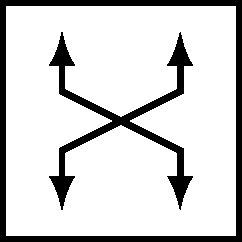
\includegraphics[width=0.9cm]{../common/fig-switch.pdf}
}
\providecommand{\router}{%
    
\includegraphics[width=0.9cm]{../common/fig-router.pdf}
}

\begin{frame}{latency (1)}
    \begin{itemize}
    \item latency: time for message: SOURCE $\rightarrow$ DEST
    \item example: \myemph<3>{1000} bit message from S to D:
    \end{itemize}
\begin{tikzpicture}
\tikzset{
    connect/.style={draw,very thick,Latex-Latex},
    computer/.style={inner sep=0mm,outer sep=0mm,execute at begin node={\computer}},
}
\node[computer,label={center:S}] (s) {};
\node[computer,label={center:D}] (d) at ([xshift=10cm]s.east) {};
\draw[connect] (s) -- (d) node[midway,above] {\myemph<2>{50 Mbit}, \myemph<3>{500 meters of copper}};
\end{tikzpicture}
\begin{itemize}
\item<2-> \myemph<2>{one} bit sent each \myemph<2>{1/50M second = 0.02 \mu s}
\item<2-> \myemph<3>{1000 bits take $0.02 \times 1000 = 20$ \mu s to sent}
    \begin{itemize}
    \item ``transmission delay''
    \end{itemize}
\item<3-> + $2.2$ microseconds for bit to go down cable ($2.3\times10^8$ m/s)
    \begin{itemize}
    \item ``propogation delay''
    \end{itemize}
\item<4-> total latency of about 22.2 \mu s
\end{itemize}
\end{frame}

\begin{frame}{latency (1, ex)}
\begin{tikzpicture}
\tikzset{
    connect/.style={draw,very thick,Latex-Latex},
    computer/.style={inner sep=0mm,outer sep=0mm,execute at begin node={\computer}},
    switch/.style={inner sep=0mm,outer sep=0mm,execute at begin node={\switch}},
}
\node[computer,label={center:S}] (s) {};
\node[computer,label={center:D}] (d) at ([xshift=10cm]s.east) {};
\draw[connect] (s) -- (d) node[midway,above] {\myemph{1 Gbit}, \myemph<3>{10 kilometers of fibre}};
\end{tikzpicture}
\begin{itemize}
\item exercise: latency for 20000 bit message from S to D
    \begin{itemize}
    \item assume speed of signal through fiber of $2.0\times10^8$ m/s
    \end{itemize}
\end{itemize}
\end{frame}

\begin{frame}{latency (2)}
    \begin{itemize}
    \item example: 1000 bit packet from S to D
    \item assume when message is received:
        \begin{itemize}
        \item 5 other 1000-bit packets in queue; no extra bits between packets
        \item no other switch processing time
        \end{itemize}
    \end{itemize}
\begin{tikzpicture}
\tikzset{
    connect/.style={draw,very thick,Latex-Latex},
    computer/.style={inner sep=0mm,outer sep=0mm,alt=<4>{label={[font=\small,label distance=0mm,text=red]south:`host'}},execute at begin node={\computer}},
    switch/.style={inner sep=0mm,outer sep=0mm,execute at begin node={\switch}},
}
\node[computer,label={center:S}] (s) {};
\node[switch] (m) at ([xshift=6.25cm]s.east) {};
\node[computer,label={center:D}] (d) at ([xshift=6.25cm]m.east) {};
\draw[connect] (s) -- (m) node[font=\small,midway,above] {50 Mbit, 500 meters of copper};
\draw[connect] (m) -- (d) node[font=\small,midway,above] {50 Mbit, 500 meters of copper};
\end{tikzpicture}
\vspace{-.5cm}
\begin{itemize}
\item S to switch, switch to D: 22.2 \mu s {\small (``propogation delay'')}
\item within switch: wait $20\times5=100$ \mu s for 5 other packets
    \begin{itemize}
    \item ``queueing delay''
    \end{itemize}
\item total latency: $22.2 + 100 + 22.2 = 144.4$ microseconds
\end{itemize}
\end{frame}

\begin{frame}{round trip time}
    \begin{itemize}
    \item round-trip-time (RTT): time for message:  \\ SOURCE $\rightarrow$ DEST $\rightarrow$ SOURCE
    \vspace{.5cm}
    \item much easier to measure than one-way latency
    \item typically how we'll set latency
    \end{itemize}
\end{frame}
